
\section{Theory}

\subsection{Basic microlensing theory}

We start by introducing in a succint manner the gravitational lensing theory that is relevant for microlensing in general and for the scope of the
present paper in particular. For a detailed presentation of the theory the reader is referred to the books and articles that represent the references
of the current section (book by Schneider and others). The general microlensing equation can be written as:
\begin{equation}
\vec{y} =   
 \begin{pmatrix}
  1-\gamma - k & 0 \\
  0 & 1 + \gamma -k \\
 \end{pmatrix} 
\vec{x} - \sum_{i=1}^{n} m_i \frac{\vec{x} - \vec{x_i}}{\left( \vec{x} - \vec{x_i} \right)^2}.
\label{eqn:microlensingequation}
\end{equation} 

The equation is valid for a set of $\it{n}$ point (Schwarzschild) lenses placed at coordinates $\vec{x_i}$. $\vec{y}$ represents the coordinates in the source plane for the respective ray, while $\vec{x}$ represents the coordinates in the lens plane. Furthermore, $\gamma$ and $k$ are the shear and surface mass density. For the lens mapping, a Jacobian can be defined:
\begin{equation} 
A(\vec{x}) = 
 \begin{pmatrix}
  \frac{\partial{y_1}}{\partial{x_1}} & \frac{\partial{y_1}}{\partial{x_2}} \\
  \frac{\partial{y_2}}{\partial{x_1}} & \frac{\partial{y_2}}{\partial{x_2}} \\
 \end{pmatrix}. 
\end{equation}
The determinant of $A(\vec{x})$ is related to the local magnification factor through the equation:

\begin{equation}
\mu(\vec{x}) = \left| \frac{1}{det(A(\vec{x}))} \right|
\label{eqn:mu_x}
\end{equation}

According to this equation, from an infinitesimally small source positioned at $\vec{x}$ in the lens plane an observed will receive a flux $\mu(\vec{x}) dF$ instead of the flux $dF$ that would be
observed in the absence of the gravitational lens. In other words the source will dim or brighten depending on whether $\mu(\vec{x})$ is subunitary or supraunitary.\\

In general, for a single infinitesimally small source more than one image can be observed, each with magnification $\mu_j$. For microlensing events the angular sizes of the
images cannot be resolved. The only observable is the flux to which all nearby images contribute. A total magnification
\begin{equation}
 \mu_t = \sum_{j} \mu_j
\end{equation}
 can be defined and account for an increase/decrease of brightness from all images.


\subsection{Magnification of a point source near a fold}

The determinant of the Jacobian $A$ can have both positive and negative values depending in which region it is computed. Such regions are well defined and separated
by critical curves where the determinant vanishes. The lens equation maps the critical curves of the lens plane into caustics in the source plane. An example of the caustic 
shape can be seen in figure \ref{fig:magnification}.\\

\begin{figure}
\centering
  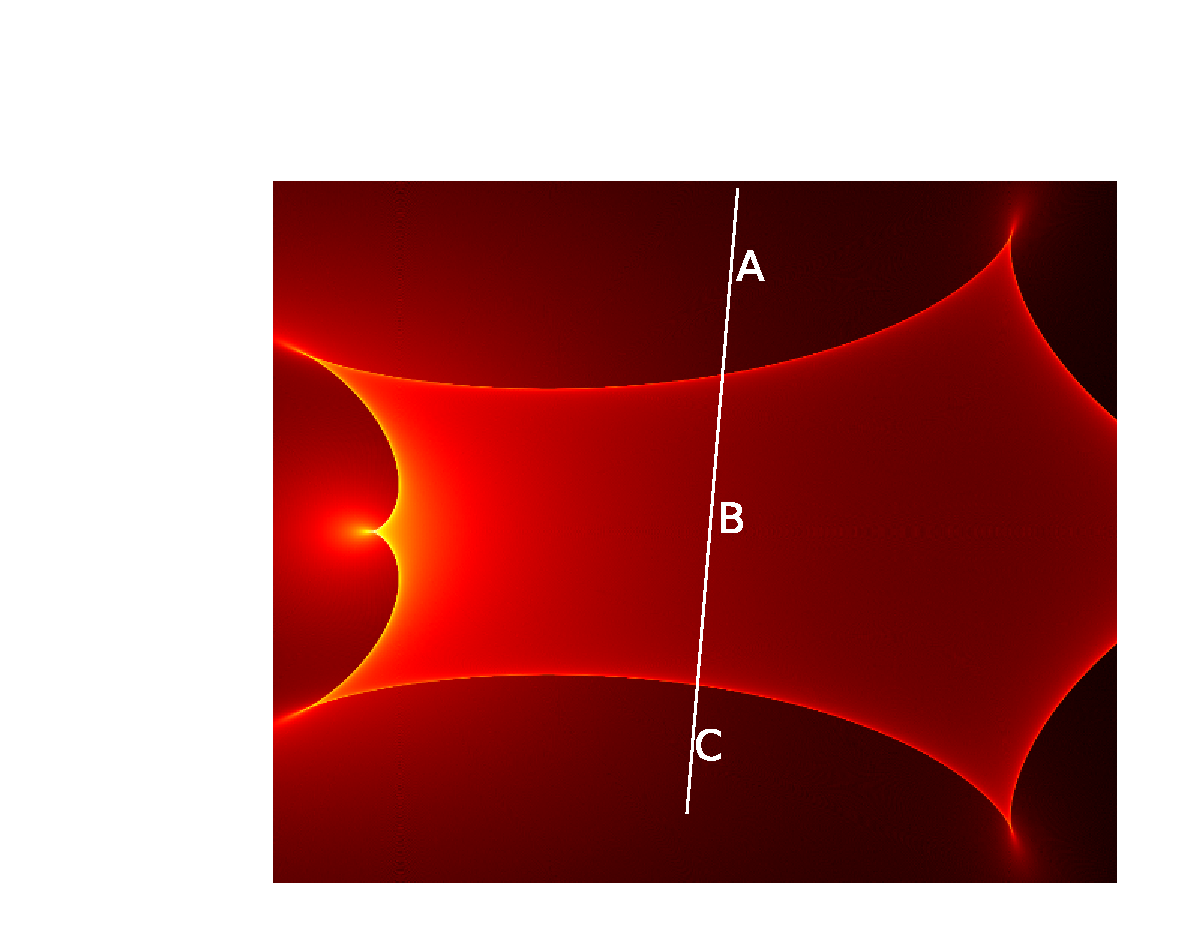
\includegraphics[width=0.95\hsize]{plots/IRIS567_path_2.eps}
\caption{\label{fig:magnification} Magnification map}
\end{figure}

Along these critical curves in the lens plane or caustics in the source plane,  the magnification $\mu$ is infinite, a result that simply follows from equation \ref{eqn:mu_x}. This statement holds only for infinitesimally small sources. For extended sources the maximum amplification is finite since only an infinitesimally small area of the source
overlaps with the caustics \citep{1986BAAS...18T.907S}. 

The matrix $A$ at the coordinates of the caustic can have rank 1 or 0. If the rank is 1 then the coordinates belong to $fold$ or $cusp$ singularities. For the purpose 
of this paper we are interested only in the behaviour around $fold$ singularities. A condition necessary to distinguish between a fold and cusp singularity is that the
eigenvector of $A$ corresponding to the null eigenvalue is not a tangent vector of the critical curve \citep{1992A&A...260....1S}(Dominik 2008).


The behaviour of the images of a point source and their corresponding magnifications near such a caustic has been thoroughly studied in the past. The reader who is interested in 
understanding the details related to this subject is referred to papers such as \cite{1986ApJ...310..568B}, \cite{1992A&A...260....1S}, \cite{2002ApJ...574..970G}, \cite{2002ApJ...580..468G}. For the present paper we only 
summarize the common result:
\begin {equation}
 \mu_{t}(p) = \mu_0 + C_0 \frac{1}{\sqrt{p}} \Theta(p).
\end {equation}
As the previous equation describes the magnification of a point source near a caustic is equal to the sum of the magnification due to other reasons $\mu_0$, assumed to be locally constant,  and a decrease with
the square root of the distance from the fold. The later term becomes activated only after the source enters the region interior to the caustic curves when the values of the stepfunction $\Theta(p)$ become unity. The proportionality
constant $C_0$  is sensible only to the local behaviour of Fermat's potential and units used for the lens plane coordinates $\vec{y}(p,q)$. 

\subsection{Magnification of an extended source near a fold}

A source of arbitrary shape can be described by a two dimensional brightness function $S_{2D}(p - p_s, q - q_s)$ defined for a coordinate system $p,q$ where $p_s, q_s$ denote the coordinates of the center of source.

For a microlensing event the lightcurve can be written for an undefined source shape as:

\begin{equation}
 F(t) = \int_{-\infty}^\infty \int_{-\infty}^\infty S_{2D}(p-p_s(t), q-q_s(t)) \mu_t(p) \mathrm{d}q \mathrm{d}p
 \label{eqn:ft2d}
\end{equation}

In order to build the previous equation we have considered that the time dependency of the flux $F$ is given only by the motion of the source with respect to a fixed caustic. Therefore the only time dependent quantities in the right hand side of the equation
are the coordinates of the center of the source $p_s,q_s$ and by construct $S_{2D}$. 

Due to the choice of the coordinate system the amplification factor has no dependence on the $q$ coordinate. The previous equation can be rewritten as:

\begin{equation}
 F(t) 
= \int_{-\infty}^\infty  \mu_t(p) S_{1D}\left(p-p_s(t)\right) \mathrm{d}p,
\label{eqn:ft}
\end{equation}
\\
where we have defined the one dimensional flux function as:
\begin{equation}
 S_{1D}(p-p_s(t)) = \int_{-\infty}^\infty S_{2D}(p-p_s(t), q-q_s(t)) \mathrm{d}q
\end{equation}

This representation is a valid approximation only when the apparent size of the source is much smaller than the corresponding Einstein angle of the lens. In this context 
all the information about the source shape and brightness that can be contained in the lightcurve is exhaustively given by the 1D flux function.
In other words, if two sources with different $S_{2D}$ have the same $S_{1D}$ they cannot be distinguished by studying their lightcurves.
 
 
\section{Models for extended sources}

In the present study we are analysing three types of sources with different surface brightness: 
\begin{enumerate}
 \renewcommand{\theenumi}{(\arabic{enumi})}
  \item a rotationally symmetric source with a bivariate gaussian surface brightness distribution,
  \item a disk source with constant surface brightness distribution,
  \item a crescent shaped source with constant surface brightness distribution.
\end{enumerate}
The first two sources are the typical choices used in the literature to describe the luminous parts of a quasar (Prasenjit should give some citations here). The third one is a recently proposed
variant \citep{2013MNRAS.434..765K}.




\subsection{Rotationally symmetric source with a bivariate gaussian surface brightness distribution}

A symmetric 2D gaussian can be described mathematically as:

\begin{equation}
 S_{2D}^G(p-p_s, q-q_s) = \frac{S_0^G}{2 \pi \sigma^2} e^{-\frac{(p-p_s)^2}{2 \sigma^2}} e^{-\frac{(q-q_s)^2}{2 \sigma^2}}.
\end{equation}
\\
The corresponding 1D brightness is:

\begin{equation}
 S_{1D}^G(p-p_s) = \frac{S_0^G}{\sqrt{2 \pi} \sigma} e^{-\frac{(p-p_s)^2}{2 \sigma^2}}.
\end{equation}
\\
Other parameters of the model are the total flux $S_0^G$ and $\sigma$. 

Although such a definition for a source would have non-zero surface/linear brightness for any coordinate $p,q$, the amount of light received by a detector from outside a $3 \sigma$ disk centered at $p_s, q_s$ 
would be insignificant. For a gaussian distributed surface brightness source the half-light radius is directly proportional to the parameter $\sigma$ according to the equation:
\begin{equation}
r_{1/2} = \sqrt{ln(4)} \sigma.
\end{equation}

\subsection{Disk source with constant surface brightness distribution}

One can construct mathematically a disk source with constant surface brightness and radius $R$ using a stepfunction:
\begin{equation}
 S_{2D}^D(p-p_s, q-q_s) = \frac{S_0^D}{\pi R^2} \Theta \left( R^2 - \left( p-p_s \right)^2 - \left( q-q_s \right)^2 \right).
\end{equation}
By integrating over $q$ coordinate the linear brightness function is obtained:


\begin{equation}
 S_{1D}^D(p-p_s) = \frac{2 S_0^D}{\pi R}  \sqrt{1 - \frac{(p-p_s)^2}{R^2} }    \Theta \left( R^2 - \left( p-p_s \right)^2 \right).
\end{equation}
\\
The half-light radius of a uniform disk source is $R/\sqrt{2}$.

\subsection{Crescent source with constant surface brightness distribution}

The surface brightness distribution of a geometric crescent can be built by considering two disk sources of constant brightness. One larger disk will contribute positively to the total flux, while one smaller disk 
that is interior to the large one will contribute negatively. This superposition can be written for 2D as:\\

\begin{equation}
 S_{2D}^C =  S_{2D}^{Dp} -  S_{2D}^{Dn}   (n+1)
 \label{eqn:s2d}
\end{equation}
with\\

\begin{equation}
 S_{2D}^{Dp}(p-p_{sn}, q-q_{sn}) = \frac{S_0^{Dp}}{\pi R_p^2} \Theta \left( R_p^2 - \left( p-p_{sp} \right)^2 - \left( q-q_{sp} \right)^2 \right)
\end{equation}
\\
and
\begin{equation}
 S_{2D}^{Dn}(p-p_{sn}, q-q_{sn}) = \frac{S_0^{Dn}}{\pi R_n^2} \Theta \left( R_n^2 - \left( p-p_{sn} \right)^2 - \left( q-q_{sn} \right)^2 \right).
\end{equation}
\\
The following notations were used: $R_p, (p_{sp}, q_{sp}), R_n, (p_{sn},q_{sn})$ are the radii and coordinate of the center for the larger positive disk and smaller negative disk respectively.  $S_0^{Dp},S_0^{Dn}$ represent the total flux of radiation received from the large and small disk. From this point forward we will not use the total flux from each source. Instead we will 
use the difference which in this case is th total flux from the crescent-shaped source $S_0^C$. \\
Equation \ref{eqn:s2d} can be written as:\\

\begin{align}
 S_{2D}^C &= \frac{S_0^C}{\pi \left(R_p^2-R_n^2 \right)} \left\{ \Theta \left[ R_p^2 - \left( p-p_{sp} \right)^2 - \left( q-q_{sp} \right)^2 \right] \right.\nonumber\\
 &\qquad \left. {} -  \Theta \left[ R_n^2 - \left( p-p_{sn} \right)^2 - \left( q-q_{sn} \right)^2 \right] \right\}.
\end{align}
\\
Analogous for the linear brightness function:

\begin{align}
 S_{1D}^C &= \frac{2 S_0^C}{\pi \left(R_p^2-R_n^2 \right)} \left\{ \sqrt{R_p^2 - (p-p_{sp})^2}  \Theta \left[ R_p^2 - \left( p-p_{sp} \right)^2 \right] \right.\nonumber\\
 &\qquad \left. {} - \sqrt{R_n^2 - (p-p_{sn})^2 } \Theta \left[ R_n^2 - \left( p-p_{sn} \right)^2 \right] \right\}.
\end{align}


There are some constraints on the parameters used to define a crescent in the previously presented manner that need to be stated. First, we must impose the obvious $R_p > R_n$ relation. Secondly, 
the small disk must always be interior to the large disk:
\begin{equation}
 R_p \ge R_n + \sqrt{\left(p_{sp} - p_{sn} \right)^2 + \left(q_{sp} - q_{sn} \right)^2}
\end{equation}

For the distances between the centers of the two disks we will use the same notations as the one found in the paper \citep{2013MNRAS.434..765K}, $a \equiv p_{sn} - p_{sp}$ and $b \equiv q_{sn} - q_{sp}$.

The half-light radius of any source is invariant to any rotational transformation. In the present case of a crescent source the effective radius is dependent on the parameters $R_p$, $R_n$ and $\sqrt{a^2+b^2}$ exclusively. From symmetry considerations the centroid of the source is colinear with the centers of the two disks and it is situated at a distance $d_c$ from the center of the brigth disk. $d_c$ can be computed numerically by solving the equation:

\begin{equation}
\frac{S_0^C}{2} =  
\end{equation}   

\section{Lightcurves of the extended sources during fold crossing}

Using equation \ref{eqn:ft} and the one-dimensional flux function presented in the previous section one can compute numerically the lightcurves of the three extented sources for the simplified 
infinite-wall-caustics model.

\subsection{Lightcurve of the gaussian source}

The amount of light received by an observer from a source with a gaussian distributed brightness with $\sigma$ and total flux $S_0^G$ in the absence of any gravitational lensing is:
\begin{equation}
 F^G(t) = \int_{-\infty}^\infty  \left( \mu_0 + \frac{C_0}{\sqrt{p}} \Theta \left( p \right) \right) \left( \frac{S_0^G}{\sqrt{2 \pi} \sigma} e^{-\frac{(p-p_s(t))^2}{2 \sigma^2}} \right) \mathrm{d}p.
\end{equation}
which can be simplified to:
\begin{equation}
 F^G(t) = \mu_0 S_0^G + \frac{C_0 S_0^G}{\sqrt{2\pi} \sigma} \int_{0}^\infty \frac{e^{-\frac{(p-p_s(t))^2}{2 \sigma^2}}}{\sqrt{p}} \mathrm{d}p.
\end{equation}


\begin{figure}
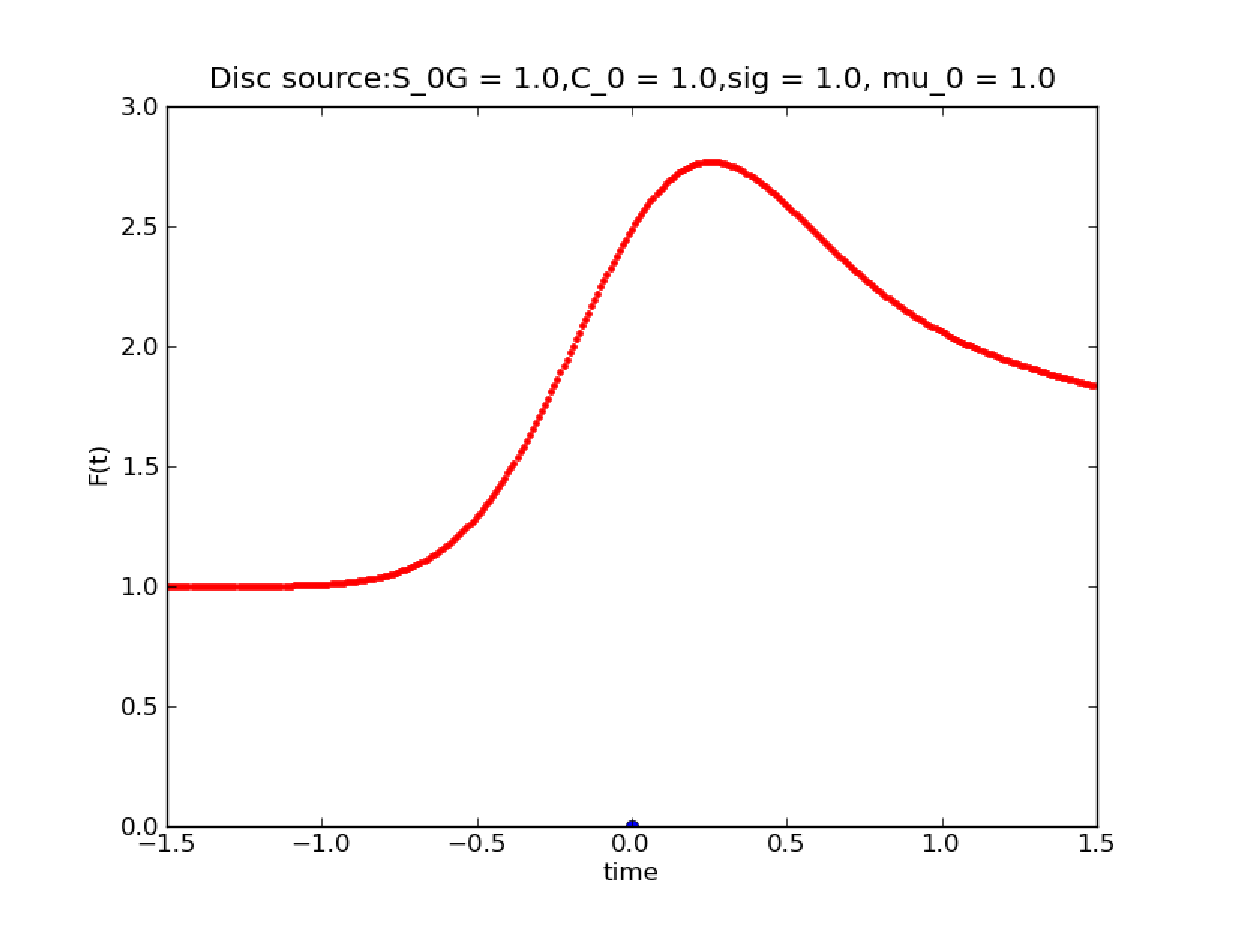
\includegraphics[width = .8\textwidth]{plots/lightcurve_gaussian_1.eps}
\caption{\label{fig:lightcurve_gauss} Lightcurve 1.}
\end{figure}


\subsection{Lightcurve of the disk shaped source}

Analogous to the gaussian shaped source, the disk source with uniform brightness, radius $R$ and unmagnified flux $S_0^D$ has a lightcurve described by the equation:

\begin{equation}
 F^D(t) = \int_{-\infty}^\infty  \left( \mu_0 + \frac{C_0}{\sqrt{p}} \Theta \left( p \right) \right) \left( \frac{2 S_0^D}{ \pi R} \sqrt{1 - \frac{\left( p-p_s(t) \right)^2}{R^2}} \Theta \left(R^2 - \left(p-p_s(t) \right)^2 \right) \right) \mathrm{d}p.
\end{equation}

which is equivalent to:
\begin{equation}
 F^D(t) = \mu_0 S_0^D + \frac{2 C_0 S_0^D}{\pi R} \int_{max(0, p_s(t) - R)}^{max(0, p_s(t) + R)} \frac{1}{\sqrt{p}} \sqrt{1 - \frac{\left( p-p_s(t) \right)^2}{R^2}} \mathrm{d}p.
\end{equation}

\begin{figure}
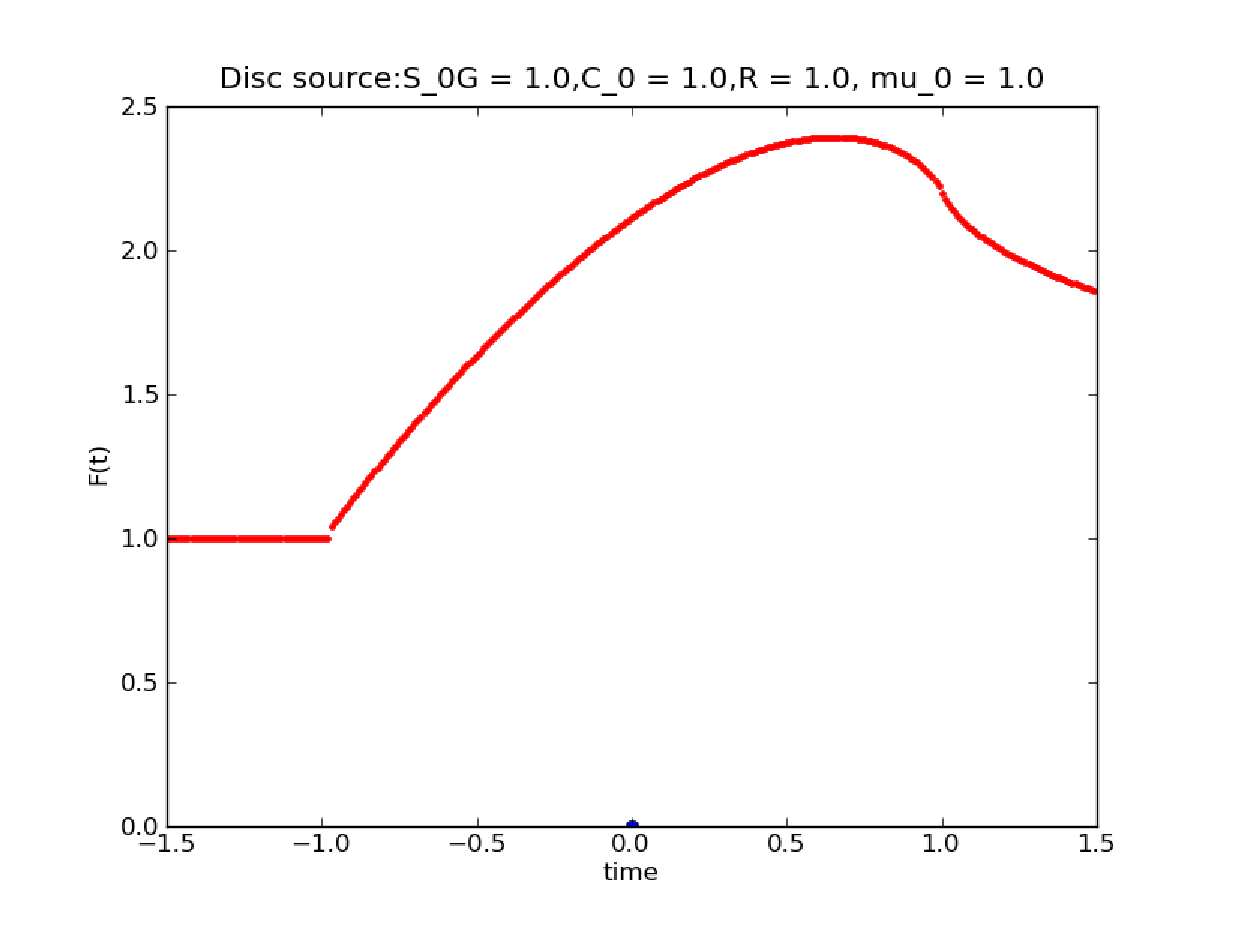
\includegraphics[width = .8\textwidth]{plots/lightcurve_disc_1.eps}
\caption{\label{fig:lightcurve_disk} Lightcurve 2.}
\end{figure}


\subsection{Lightcurve of the crescent shaped source}

The lightcurve of a crescent shaped source with unamplified flux $S_0^C$, radii $R_p$, $R_n$ and center displacement $a(t)$ is:
\begin{equation}
 F^c(t) = \mu_0 S_0^C + C_0 \frac{2 S_0^C}{\pi \left( R_p^2 -R_n^2 \right) } 
\left(\int_{max(0, p_s(t) - R)}^{max(0, p_s(t) + R)} \sqrt{\frac{R_p^2 - \left( p-p_s(t) \right)^2 }{p}} \mathrm{d}p 
  -  \int_{max(0, p_s(t) - a(t) - R)}^{max(0, p_s(t) -a(t) + R)} \sqrt{\frac{R_p^2 - \left( p-p_s(t) +a(t) \right)^2 }{p}}  \mathrm{d}p \right)
\end{equation}


\begin{figure}
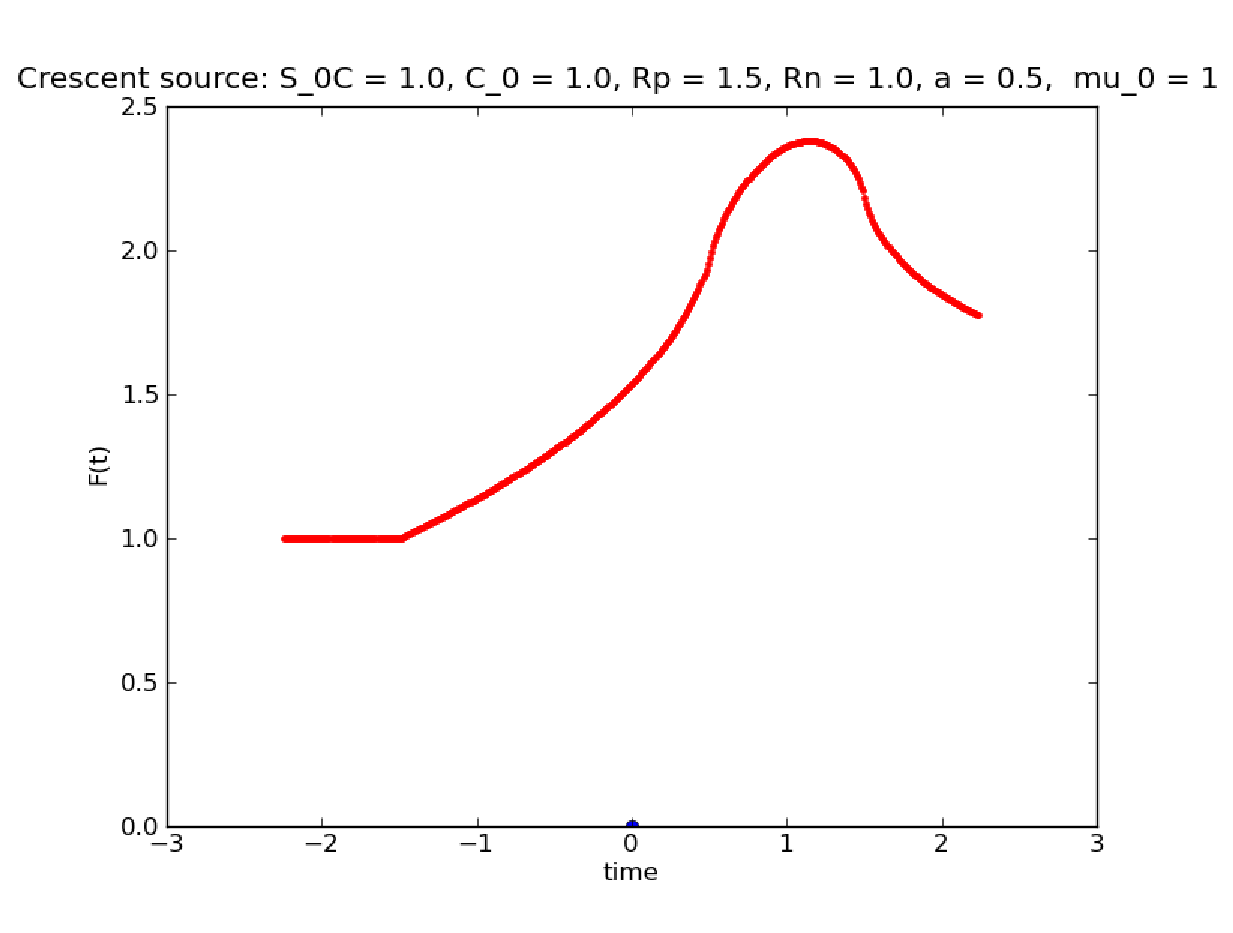
\includegraphics[width = .8\textwidth]{plots/lightcurve_crescent_1.eps}
\caption{\label{fig:lightcurve_crescent} Lightcurve 3.}
\end{figure}

The function $p_s(t)$ can be chosen to be equal to $v_p(t-t_0) + p_{s0}$. Where $p_{s0}$ is the coordinate $p$ of the source at the initial time, and $v_p$ is the component of the velocity
along the $p$ axis. Such a modeling of the motion of the object in the source plane describes a linear motion with constant velocity. Furthermore, we reduce the complexity of the model by 
chosing the function $a(t)$ to be constant in time.  


